\chapter{Data verwerking}
% inleiding van dit hoofdstuk, wat ga ik allemaal bespreken
% bespreken benodigdheden duidelijke resultaten
In dit hoofdstuk wordt de data verkregen uit vorig hoofdstuk verwerkt in visuele resultaten. De verschillende ondernomen stappen worden besproken. De eerste stap behandelt het verwerpen van bepaalde datapunten. Vervolgens wordt de data met bepaalde parameters in verband gebracht. En tot slot wordt de data op vlak van spreiding geanalyseerd en uiteindelijk in grafiekvorm weergegeven. De resultaten zelf worden in hoofdstuk \ref{ch:resultaten} besproken. 

\section{Data cleaning}
Een belangrijk gebeuren voor de data verwerkt kan worden, is het schoonmaken van de data. Tijdens het uitvoeren van metingen is het mogelijk dat er meetfouten plaatsvinden. Deze kunnen door allerlei oorzaken plaats vinden en moeten zo veel mogelijk vermeden worden. In deze sectie bespreken we een aantal van deze meetfouten en hoe deze aangepakt en verwerkt worden. 
% verwerpen van data in vorig hoofdstuk,
% voorbeeld van verworpen data weergeven.
% deel dat al in data verwerving is gebeurd(selectie data)
	\subsection{Verwerpen data}
	Een eerste wijze van schoonmaken is het verwerpen van datapunten waarvan er geweten is dat deze onmogelijk correct kunnen zijn. Dit betreft meetfouten waar bijvoorbeeld de duur van het uitvoeren van een programma gelijk is aan nul seconden. Dit is uiteraard niet mogelijk, elke meting heeft namelijk een duur van bepaalde grootte. Een andere meetfout die geregeld op trad kwam bij het meten van het \gls{cpu}-verbruik voor. Indien na het uitvoeren van een programma bleek dat er geen activiteit in de \gls{cpu} werd gemeten is dit als gevolg van een meetfout. 
	
	Indien deze meetfouten worden gedetecteerd zal de volledige meting worden verworpen en wordt de meting herhaald. De controle op deze meetfouten vindt dus plaats na het uitvoeren op de meting en voor het opslaan van de data. In listing \ref{lst:meetfout} kan deze controle teruggevonden worden. Alleen nadat er geen meetfout gedetecteerd wordt de data uitgeschreven en wordt de iteratie erkend als een geldige iteratie. Door een imperfecte meting te hernemen blijft het totaal aantal bruikbare datapunten bijgevolg altijd 20.
	
	\newpage
	
	\begin{lstlisting}[caption={Controleren op meetfouten.}, captionpos=b,label={lst:meetfout}]
# Meting wordt gecontroleerd voor 
if (mean(cores) != 0.0) and (time_stop-time_start != 0):
	logging_data(10, time_stop, time_start, cores)
	iteration += 1
print("iteration: ", iteration, " mean cores: ", mean(cores), " duration: ", time_stop-time_start)
\end{lstlisting}
	
	
	\subsection{Behandelen uitschieters}
	De tweede wijze waarop de data wordt schoon gemaakt is door het behandelen van uitschieters. Tijdens het meten is het mogelijk dat een datapunt verder of dichter van het gemiddelde licht door een externe factor. Zo kan bijvoorbeeld een subroutine van het Operating System de meting vertragen en hierdoor de meting be\"invloeden. Om deze invloeden te vermijden is het nodig om de uitschieters of outliers te herkennen en te elimineren. Outliers worden hier beschouwd als datapunten die een grotere afwijking van het gemiddelde hebben dan drie standaardafwijkingen. Om deze outliers te vinden wordt er een boxplot opgesteld met behulp van de module matplotlib. In figuur \ref{fig:outliers} kan een voorbeeld van data met een outlier gevonden worden. Zodra de voornaamste outliers ge\"identificeerd zijn, zullen deze aangepast worden. De data wordt veranderd in het gemiddelde van de overige niet-uitschieters om het gemiddelde van de ware data niet te wijzigen. 

	\begin{figure}
		\centering
		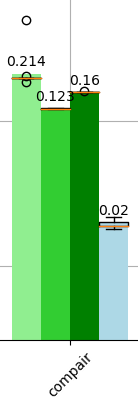
\includegraphics{afbeeldingen/outliers.png}
		\caption{Een voorbeeld van uitschieters in data van de duur van het compairprogramma.}
		\label{fig:outliers}
	\end{figure}

\section{Vormgeving resultaten}
% wat zijn de gewenste resultaten (-vormen)
	% verschillende parameters uit show_plot(): log, boxplot, normalise
	% Hoe simpeler hoe beter
In deze sectie wordt er besproken uit welke grootheden de resultaten zullen bestaan, hoe deze gevormd worden en op welke manier de resultaten gevisualiseerd worden. 

De belangrijkste te onderzoeken parameter is de tijd. De duur van uitvoeren dat een programma in beslag neemt kan een grote factor spelen bij het maken van een kosten-baten analyse. Echter als er enkel de latency met elkaar vergeleken wordt, kan dit leiden tot een vertekend beeld. Daarom worden ook factoren zoals \gls{cpu}-gebruik en kloksnelheid in rekening gebracht. De latency per percentage \gls{cpu}-gebruik en per MHz kloksnelheid geeft een beter beeld van de performantie van elk toestel. Een andere variabele die in rekening gebracht kan worden is het vermogen dat elk toestel verbruikt. Door de latency te vermenigvuldigen met het vermogen bekomt men de energie die verbruikt wordt tijdens de executie. Voor de grootheden geldt:

\begin{equation}
	time \cdot power = s \cdot \frac{J}{s} = J = Energy	
\end{equation}

Het is interessant om de verbruikte energie van de verschillende toestellen voor hetzelfde programma met elkaar te vergelijken. Toepassingen die energie gebonden zijn of waar een batterij de voeding voorziet kunnen een afweging maken tussen het energieverbruik en de duur van executie.

\section{Overzicht code}
% Uitleg code plot results






